% For more detailed article preparation guidelines, please see:
% http://f1000research.com/author-guidelines

\documentclass[10pt,a4paper]{article}
\usepackage{f1000_styles}
\usepackage{gensymb}

%% Default: numerical citations
\usepackage[numbers]{natbib}

%% Uncomment this lines for superscript citations instead
% \usepackage[super]{natbib}

%% Uncomment these lines for author-year citations instead
% \usepackage[round]{natbib}
% \let\cite\citep

\usepackage{nicefrac}
\usepackage{url}
\def\UrlBreaks{\do\/\do-}

% Can turn off hyperref if it unwanted, but it is generally useful IMO
\usepackage{xr-hyper}
\usepackage{hyperref}

%\usepackage{xr} % external references (uncomment if not using xr-hyper)
\externaldocument[main]{main}

\begin{document}

\title{Supplemental Material for:\\
Evaluation of predicted Medfly (\textit{Ceratitis capitata}) quarantine length in the United States utilizing degree-day and agent-based models}

\author[1,2]{Travis C. Collier}
\author[1,3]{Nicholas C. Manoukis}
\affil[1]{Daniel K. Inouye US Pacific Basin Agricultural Research
Center (PBARC), United States Department of Agriculture,
Agricultural Research Service,
Hilo, Hawaii, 96720, USA}
\affil[2]{corresponding author; email: Travis.Collier@ARS.USDA.gov}
\affil[3]{email: Nicholas.Manoukis@ARS.USDA.gov}
% Please list all authors that played a significant role in the research involved in the article. Please provide full affiliation information (including full institutional address, ZIP code and e-mail address) for all authors, and identify who is/are the corresponding author(s).

\maketitle
\thispagestyle{fancy}

%\begin{abstract}
%\end{abstract}

%\section*{Keywords}

\tableofcontents

\clearpage

%%%%%%%%%%%%%%%%%%%%%%%%%%%%%%%%%%%%%%%%%%%%%%%%%%%%%%%%%%%%%%%%%%%%%%%%%%%

\section{``Supernorm'' figures}

\subsection{Daily normal of hourly temperatures}
\begin{figure*}[hb!]
\centering
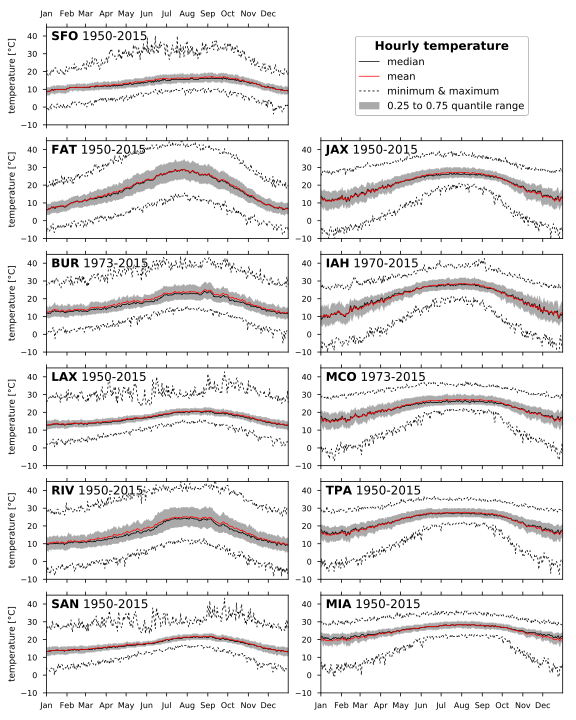
\includegraphics[width=1.0\textwidth]{figs/fig_all_hourly_temps_supernorm.pdf}
\caption{\label{fig:temperature_supernorm}
Hourly temperature data aggregated by day of year.
}
\end{figure*}
\clearpage

\subsection{Degree day based PQL supernorm}
\begin{figure*}[hb!]
\centering
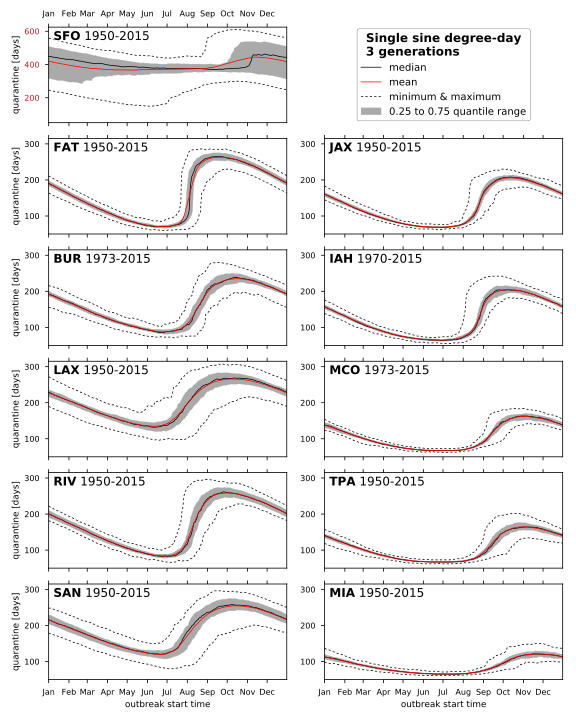
\includegraphics[width=1.0\textwidth]{figs/fig_all_BMDD_supernorm.pdf}
\caption{\label{fig:ddPQL_supernorm}
Single sine degree day based predicted quarantine lengths aggregated by day of year.
}
\end{figure*}
\clearpage

\subsection{MED-FOES PQL based supernorm}
\begin{figure*}[hb!]
\centering
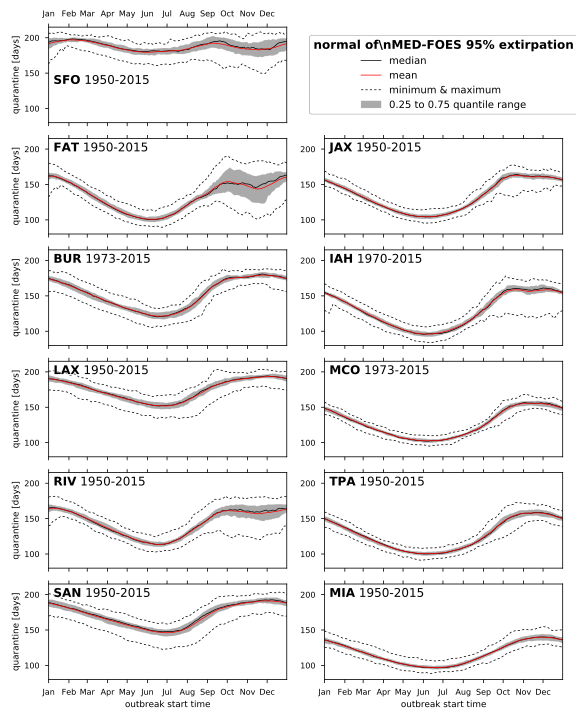
\includegraphics[width=1.0\textwidth]{figs/fig_all_pe95_supernorm.pdf}
\caption{\label{fig:medfoesPQL_supernorm}
MED-FOES based predicted quarantine lengths aggregated by day of year.
}
\end{figure*}
\clearpage


\subsection{Bar1}
\subsubsection{cat1}

\subsection{Bar2}

\section{Foo2}

%%%%%%%%%%%%%%%%%%%%%%%%%%%%%%%%%%%%%%%%%%%%%%%%%%%%%%%%%%%%%%%%%%%%%%%%%%%

\begin{figure}[ht!]
\centering
\includegraphics[width=0.4\textwidth]{figs/sitemap.pdf}
\caption{\label{fig:sitemap}Location of sites analyzed.}
\end{figure}

\begin{table*}[ht!]
\hrule \vspace{0.1cm}
\caption{\label{tab:sites}Weather station (NOAA ISD) sites used.}
\centering
\begin{tabledata}{llllrrrl}
\header Callsign & Station Name & State & Latitude & Longitude & Elevation & Start year \\
\row KSFO &  SAN FRANCISCO INTERNATIONAL A &  CA &  +37.620 &  -122.365 &  2.4 & 1950 \\
\row KFAT &  FRESNO YOSEMITE INTERNATIONAL &  CA &  +36.780 &  -119.719 &  101.5 & 1950 \\
\row KBUR &     BURBANK-GLENDALE-PASA ARPT &  CA &  +34.201 &  -118.358 &  236.2 & 1973 \\
\row KLAX &  LOS ANGELES INTERNATIONAL AIR &  CA &  +33.938 &  -118.389 &  29.6 & 1950 \\
\row KRIV &         MARCH AIR RESERVE BASE &  CA &  +33.900 &  -117.250 &  468.2 & 1950 \\
\row KSAN &  SAN DIEGO INTERNATIONAL AIRPO &  CA &  +32.734 &  -117.183 &  4.6 & 1950 \\
\row KJAX &  JACKSONVILLE  INTERNATIONAL A &  FL &  +30.495 &  -81.694 &  7.9 & 1950 \\
\row KIAH &  G BUSH INTERCONTINENTAL AP/HO &  TX &  +29.980 &  -95.360 &  29.0 & 1970 \\
\row KMCO &  ORLANDO INTERNATIONAL AIRPORT &  FL &  +28.434 &  -81.325 &  27.4 & 1973 \\
\row KTPA &    TAMPA INTERNATIONAL AIRPORT &  FL &  +27.962 &  -82.540 &  5.8 & 1950 \\
\row KMIA &    MIAMI INTERNATIONAL AIRPORT &  FL &  +25.791 &  -80.316 &  8.8 & 1950 \\
\end{tabledata}
\end{table*}




The MED-FOES data is summarized here by the number of days from the start date required for
95\% of the simulations in a run to be eradicated, referred to as pe95.

\subsection*{Statistical analysis}

The main results reported here are `normals' in a meteorological sense of term,
but without the typical running mean smoothing which would complicate
interpretation of the results.
For a variable of interest (eg. temperature or PQL), 
all values for the same calendar day irrespective of year (eg. 20-July) are
aggregated and summary statistics such as mean, minimum, maximum, and standard deviation 
are computed for each aggregation.
Figure \ref{fig:main_summary} shows 
the mean of the normal PQL based on 3 generation degree day accumulation 
and MED-FOES 95\% extirpation
along with the minimum and maximum of the normals for temperatures.
Figures \ref{fig:DD_variation_summary} and \ref{fig:pe95_variation_summary} show the 
standard deviations ($\sigma$) of the normals for the degree day and MED-FOES based PQL.
\texttt{Temperature functions.ipynb} contains the code used to perform normal calculations, 
and the code generating these figures is \texttt{Summary Figures.ipynb}.

The results reported here are the normals of PQL computed using the full temperature time series
as opposed to computing PQL from the normal of the temperature timeseries.
While the latter is fairly common practice, it is not mathematically proper 
since, as with means, the normal of a function of $X$ is not generally equal to the function applied to the normal of $X$.
Additionally, by computing the normals of the predicted quarantine durations, 
we can investigate properties of the distribution of values as shown in 
figures \ref{fig:DD_variation_summary} and \ref{fig:pe95_variation_summary} 
and the ``supernorm" supplemental figures.

%\subsection*{Historical quarantines}
%
%%\begin{figure}[ht!]
%%\centering
%%\includegraphics[width=0.4\textwidth]{figs/fig_historic_quarantines.pdf}
%%\caption{\label{fig:historic_quarantines}
%%Day-of-year timing and size of historic Medfly quarantines in CA.
%%SFO 1980 and LAX 1991 were very long duration outliers.
%%Quarantines before the preventative release program was initiated in 1994 are denoted by `X's.
%%}
%%\end{figure}
%
%A list of 34 Medfly quarantines in CA dating from 1975 to early 2017 was obtained from 
%APHIS\cite{??}.  
%Each quarantine location was associated with a site from the 11 sites analyzed here.
%For a number of the historic quarantines, this is a rough association since temperature/climate
%can vary significantly over a short distance, especially between coastal and more 
%inland locations.
%Temperature data from the nearest site and the historic quarantine start date was used to 
%compute the 3 generation degree-day duration along with MED-FOES 95\% extirpation.
%PQLs were also computed using the day-of-year of the historic quarantines 
%and the mean of the normal PQL values for the nearest site.
%Values are reported in the supplemental table ??.
%%\ref{fig:historic_quarantines}

\section*{Results}

\begin{table}[htb!]
\hrule \vspace{0.1cm}
\caption{\label{tab:variance_captured_by_normal}
Percentage of PQL variance captured by the mean of the normal.  
DD PQL is the 3 generation single sine degree day based prediction, 
and pe95 is the MED-FOES agent-based simulation predictions.}
\centering
\begin{tabledata}{lrr}
\header & \multicolumn{2}{c}{$R^2$} \\
\header Site & DD PQL & pe95 \\
\row SFO &   9.12\% & 28.01\% \\
\row FAT &  93.93\% & 75.68\% \\
\row BUR &  90.71\% & 90.88\% \\
\row LAX &  80.17\% & 83.07\% \\
\row RIV &  92.23\% & 81.89\% \\
\row SAN &  80.99\% & 80.91\% \\
\row JAX &  96.45\% & 94.78\% \\
\row IAH &  95.10\% & 91.80\% \\
\row MCO &  94.62\% & 95.77\% \\
\row TPA &  91.91\% & 94.40\% \\
\row MIA &  88.42\% & 92.00\% \\
\end{tabledata}
\end{table}

There is significant variation in PQL across both time and location.
The temporal variation in PQL is dominated by a yearly cycle
which is characterized well by the normal values shown in figure \ref{fig:main_summary}.
Table \ref{tab:variance_captured_by_normal} shows the percentage of variance in 
quarantine length predictions which is captured by the mean of the normal yearly cycle (aka. $R^2$) for each site.
At all but one site, greater than 75\% of the variance in both degree day and MED-FOES based PQL
is accounted for by the mean normal, and the majority exceed 90\%.
SFO is an exception to the overall rule, with the mean normal accounting for only 9.1\% of the variation in 
degree day based PQL and 28.0\% of the MED-FOES based PQL.
This is also shown in the respective `supernorm' supplemental figures S?? and S??.

\subsection*{Seasonal dependence}

The seasonal variation, evidenced by the general shape of the curves shown in figure \ref{fig:main_summary}, 
is doubtless familiar to anyone engaged in Medfly pest management.
Outbreaks starting in the late summer, autumn, or early winter will extend through relatively cold periods
where thermal dependent development will be slow and therefore extend the duration of quarantine required
for 3 generations of degree days to accumulate (referred to as DD PQL hereafter).
Similarly, outbreaks starting in the spring or early summer often lead to short quarantines due
to the relatively high temperatures.

This familiar pattern is also predicted by the MED-FOES ABS despite it being 
quite different in nature from simple degree day accumulation.
However, the MED-FOES predictions (pe95) show a smaller seasonal swing.
pe95 generally produces a smaller overall range of PQLs,
with longer quarantines than DD PQL for spring and early summer outbreaks,
and shorter quarantines for late summer through early winter.

A particular feature of interest, shown most dramatically at FAT in figure \ref{fig:main_summary},
is that MED-FOES PQL often flattens out or even dips for quarantines starting in the late 
autumn or early winter.  This can be due to relatively rare and brief cold-snaps,
normally lasting only a few hours, which increase mortality.
Since DD PQL does not account for mortality, it misses the effect of cold-snaps entirely.
This cold-snap effect is most clearly seen at more northern and 
more inland sites where cold-snaps are more likely: 
particularly FAT and RIV, but also BUR, LAX, JAX, and IAH.

\subsection*{Geographic dependence}

\begin{figure*}[ht!]
\centering
\includegraphics[width=0.9\textwidth]{figs/fig_latitude_trend_withSFO.pdf}
\caption{\label{fig:latitude_trend} Predicted quarantine length dependence on latitude.
For each site, the mean, median, and inter-quartile range are shown (similar to a boxplot).
An ordinary least-squares linear fit to the median values is shown by the green lines.
The left pane is for single sine degree day predictions,
and MED-FOES based predictions are in the right pane.
}
\end{figure*}

PQL generally shows a positive correlation with latitude\cite{??}.
Sites are ordered by latitude in the figures and tables.
As seen in figure \ref{fig:main_summary}, higher latitude sites tend to have longer PQL 
as well as larger seasonal swings for both DD and MED-FOES based predictions.

Figure \ref{fig:latitude_trend} shows the relationship between PQL and latitude.
An ordinary least squares fit to the median PQL at each site shows a significant slope for
both DD ($F{=}14.08$, $p{=}0.005$) and MED-FOES ($F{=}10.55$, $p{=}0.010$), but
the DD based predictions are more sensitive to latitude than MED-FOES
(coefficients of 17.39 and 4.78 respectively).
Additionally, MED-FOES predictions are better behaved for SFO, and to a lesser extent FAT, 
where the DD model for Medfly appears to break down.

In addition to the variation associated with latitude, 
large differences in PQLs computed for the same start date 
can exist between even relatively nearby sites.
For example, the differences in both degree day and MED-FOES PQLs 
for the three sites in the Los Angeles region (LAX, BUR, RIV) 
(shown in the supplemental figure \ref{sfig:??})
show a strong seasonal component with a spike in July and/or August.
The difference in DD PQL between LAX and BUR is normally about a month
(overall median=35 days; overall 25\% \& 75\% quantiles are 28 \& 45 days), 
but the median difference of the normal exceeds 75 days in August with some 
PQL differences up to 142 days.
Differences in MED-FOES PQLs are more seasonally stable, 
with the LAX minus BUR difference not exceeding 42 days at its maximum.


\subsection*{Variance and uncertainty}

\begin{figure*}[ht!]
\centering
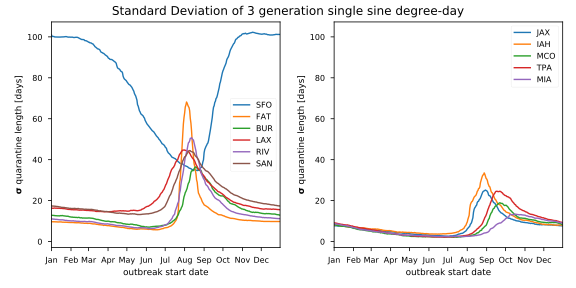
\includegraphics[width=0.9\textwidth]{figs/fig_BMDD_variation.pdf}
\caption{\label{fig:DD_variation_summary}Variation in quarantine length prediction 
based on 3 generations of single-sine degree day accumulation.}
\end{figure*}

\begin{figure*}[ht!]
\centering
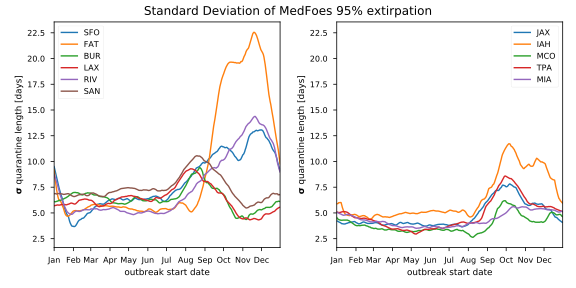
\includegraphics[width=0.9\textwidth]{figs/fig_pe95_variation.pdf}
\caption{\label{fig:pe95_variation_summary}Variation in quarantine length prediction 
based on 95\% of MED-FOES simulations showing extirpation.}
\end{figure*}


Figures \ref{fig:DD_variation_summary} and \ref{fig:pe95_variation_summary}
report the standard deviation ($\sigma$) of the normal for DD PQL and MED-FOES PQL 
respectively.
These indicate the year to year variability of the PQL for outbreaks starting at a
given time of the year and can be used to gauge the uncertainty of quarantine 
length predictions relative to the actual quarantine length which will be required.
Similar information is represented by the inter-quartile ranges 
shown in figure \ref{fig:latitude_trend} and the `supernorm' supplemental figures.
Those `supernorm' figures also show that the underlying distributions of PQL 
values are generally not highly skewed, making $\sigma$ a relatively easy to interpret 
proxy for uncertainty.

Excluding SFO, the mean normal is a good predictor of DD PQL with values below 20 days
except for the late summer and early autumn, where variance increases 
due to quarantines extending through the cold season.
FAT and, to a lesser extent, RIV show this increase more dramatically, presumably due to their more 
arid/inland climates where both daily and seasonal temperature ranges are larger
(also see figure \ref{fig:main_summary}).
The standard deviation generally decreases with latitude.

The standard deviation in DD PQL for SFO shows a inversion of the seasonal trend 
other sites exhibit.
This is due to the colder temperatures leading to extremely long degree day based 
quarantine predictions frequently extending across two winter seasons.

The standard deviations of MED-FOES based PQL normals 
shown in figure \ref{fig:pe95_variation_summary}
are generally about \nicefrac{1}{2} as large as for DD based PQL.
This indicates that MED-FOES PQL not only shows less dramatic seasonal swings, 
but is also produces more consistent predictions across years.
Values again generally decrease with latitude, but less consistently than DD PQL $\sigma$ of normals.
Also, unlike with the DD PQL, the results for SFO appear consistent with other sites.

A notable feature is that BUR, LAX, and SAN all show an increase in the year to year variation
in MED-FOES PQL starting in July and extending through November, 
while that increase for all other sites starts in July or August 
but extends all the way to January or February.
Additionally, results for FAT show a sharp increase in uncertainty starting in September, fitting with the 
more aird/inland climate.  RIV shows a significant but more gradual increase.

\subsection*{Extrapolation from historical quarantines}

A list of 34 Medfly quarantines in CA dating from 1975 to early 2017 was obtained from 
APHIS\cite{??} and is shown in the supplemental table ??.
All but two of these quarantines were declared in the latter half of the year
(July through December) where DD PQLs are typically relatively long,
with 68\% ($23/34$) occurring in September through October where DD PQLs are
longest. 
August, the month where uncertainty in DD PQL often spikes 
(see figure \ref{fig:DD_variation_summary}), 
accounts for 30\% ($7/34$) of historic quarantines.

DD and MED-FOES based PQLs were computed using the start date for each historic
quarantine and the temperature data from the closest site of the 11 analyzed
here (see supplemental table ??).
For this set of hypothetical quarantines, 
MED-FOES produced significantly shorter quarantines
(mean=169.7 days, $\sigma$=21.8 days)
than simple 3 generation DD accumulation
(mean=234.2 days, $\sigma$=79.2 days)
(t-statistic=6.01, $p<10^{-5}$).
Additionally, the variance in the difference between quarantine lengths
using a specific date and the mean of the normal PQL for that day of year
were smaller for MED-FOES ($\sigma$=8.2 days)
than with DD ($\sigma$=25.9 days)
(F-statistic=9.92, $p<10^{-8}$).

% @ TCC Maybe for supplemental...
%\begin{table}[htb!]
%\hrule \vspace{0.1cm}
%\caption{\label{tab:histoirc_quarantine_PQL}
%}
%\centering
%\begin{tabledata}{lrrr}
%\header & 
%\vtop{\hbox{\strut DD PQL $-$}\hbox{\strut normal}} &
%\vtop{\hbox{\strut MED-FOES PQL $-$}\hbox{\strut normal}} &
%\vtop{\hbox{\strut DD PQL $-$}\hbox{\strut MED-FOES PQL}} \\
%%\header & DD PQL - normal & MED-FOES PQL - normal & DD PQL - MED-FOES PQL\\
%\header & \multicolumn{3}{c}{[days]} \\
%\row N        & 34    & 34    & 34    \\
%\row mean     & -6.4  & -0.6  & 64.5  \\
%\row $\sigma$ & 25.9  & 8.2   & 62.6  \\
%\row min      & -77.7 & -22.9 & -40.1 \\
%\row 25\%     & -17.5 & -2.7  & 39.0  \\
%\row 50\%     & -4.7  & -0.5  & 67.0  \\
%\row 75\%     & 11.5  & 3.3   & 93.6  \\
%\row max      & 36.1  & 16.4  & 191.8 \\
%\end{tabledata}
%\end{table}




\section*{Discussion}
% The discussion should include the implications of the article results in view of prior work in this field.

The principal contributions of this work can be broken down into three categories: 
1) Comparison of PQLs as determined by the DD and ABS methods. 
2) variation in average PQLs across time of year and space, and
3) variation in PQLs within a time of year and location.
Consideration of all three of these by program managers, planners and other decision makers 
is likely to improve quarantines by informing resource allocation ahead of outbreaks, reducing 
quarantine costs in some cases, and reducing risk from premature quarantine suspension in others. 
The results presented cover most of the latitudinal range 
of Medfly suitability within the United States 
as well as many sites of probable introduction,
and will hopefully find use as a general guide.

% overall comparison of DD and ABD PQLs here.

Extirpation models are extremely difficult to test for accuracy given 
the impracticality of experimental introductions and 
the sparse and idiosyncratic nature of historic outbreaks.

Requiring a fixed number (typically 3) generations of degree days to pass is 
a "tried and true" method, but not explicitly an extirpation model.
It may overestimate required quarantine length through cold weather\cite{??}
and may underestimate length when growth conditions are very favorable, 
which somewhat paradoxically leads to quicker extirpation under SIT.
%However, the simplicity of degree day and the "has worked so far" nature
%means it will likely continue to be the regulatory benchmark.

ABS results may be used to inform and modulate responses and treatments which are under
the discretion of managers.
In situations where DD PQL greatly exceed those from MED-FOES, it is likely
that DD is missing important effects such as cold snaps which may justify
shortening quarantine periods.
On the other hand, in cases where MED-FOES predicts longer times to extirpation, it
is plausible that the DD model is overly generous and 
eradication treatments and SIT releases should be conducted aggressively.


A few specific results arising from overall comparisons of different locations are worth highlighting. 
In general, DD PQL for Medfly 
generated from San Francisco International Airport temperature data
 are almost certainly too long for the entire year.
The ABS PQLs are flatter and seem more realistic at around 200 days for San
Fransisco compared with the 400-550 days of DD PQLs. 
For several other California locations (typified by Fresno and 
Riverside) DD PQLs are in close alignment with those from the ABS 
for the first half of the year 
but go significantly longer in the cooler months. 
For three of four Florida locations analyzed, 
DD PQLs are significantly shorter than the ABS results
 (Miami, Tampa, and Orlando).
The extent of the difference in those Florida locations is smaller in the later months of the year,
but the generality of this pattern suggests that the margin of safety for quarantines as 
calculated by DD in those locations may be smaller than expected. 

Other systematic comparisons of (PQLs? development?) include .. (PLUG Davis paper here) 
% Are there other papers we should compare with here? I would guess yes...


As expected, there is significant variation in PQL depending on the location of the outbreak, 
with the extremes in our study sites represented by Miami and San Francisco.
These geographic results could be
compared directly to previous efforts to model climatic suitability of different parts of the US 
for Medfly, by equating longer PQLs with higher climatic suitability.
One of the early studies on the subject focused on Medfly found higher climatic suitability in 
Florida locations (Fort Pierce and Orlando) compared with California 
sites \cite{messenger_bioclimatic_1954}. 
Within California, however, those authors found a higher number of suitable months in coastal 
areas such as Oceanside compared with Riverside and Fresno, roughly paralleling our 
findings (compare Los Angeles or San Diego with Fresno or Riverside).
A more recent analysis of climatic suitability likewise concludes that coastal 
S. California is the most favorable area of the state for Medfly, but 
favorability drops inland in the south due to desert conditions.
Suitability in central and northern California is limited by cold temperatures and 
freezes \cite{gutierrez_assessing_2011}. 


Seasonal variation within locations revealed WORDS ON SEASONAL HERE
[
Anna's 2014 paper; refs she cites "It is well documented in regional studies from several areas of the world that Medfly has a highly seasonal pattern to its population dynamics"...:
https://www.ncbi.nlm.nih.gov/pmc/articles/PMC4222914/
]


% variation within location/time
An important aspect of PQLs from the ABS is variation within particular times of years and locations. 
Rare events like cold snaps can increase mortality in the ABS,
and thereby lead to shorter PQLs than expected based on historical averages, or DD PQLs.
The specificity of the ABS is particularly useful in determining 
when quarantines might be safely suspended due to a rare event,
something that would not be captured by the DD model.
The DD model includes only development for generating PQLs,
and development is halted at low temperatures, extending quarantine lengths.
The ABS, however, also includes mortality for generating PQLs,
which means that low temperatures can significantly reduce estimates.
% perhaps name names of locations
% where the variation is particularly acute (like FAT?)
% Possibly put a paragraph on variation in PQLs seen in figs 3,4- patterns different for ABS vs DD

In Calfornia, historically quarantines have most frequently occurred at times of year when 
DD based quarantines are drawn out by cold weather and the MED-FOES ABS model predicts significantly
shorter durations.
Furthermore, 30\% of those historic quarantines happened in August where there is a great 
deal of uncertainty in forward predictions of DD quarantine durations based on normal values.
If we assume those historic CA quarantines are a guide, the ABS model would very likely
produced more predictable and shorter quarantine durations for future outbreaks.



%%%%%

By expanding on previous work \cite{manoukis_agent-based_2014}, this study suggests that an 
improved approach to setting quarantine lengths would 
include estimates from the DD method and from the ABS.

The initial quarantine length estimate could be quickly produced based on the distribution of PQL values
generated using historical temperatures.
This would generate not just a single 'typical' value as the current method of projecting
using historical average/normal temperatures does.
The median 'most likely' value may be used for official estimates, while
the variance and extremes would provide managers and affected parties additional
information vital for planning.



Once the eradication program is underway, weekly simulations
via the ABS could indicate the likelihood that extirpation has been achieved. If the threshold 
95\% extirpation is observed the decision to end quarantine early could be made, or in the case 
where the ABS has not reached the 95\% threshold at the end of the DD PQL additional measures could 
be considered to reduce the risk of re-detection.


%\section*{Conclusions}
%Please state what you think are the main conclusions that can be realistically drawn from the findings in the paper, taking care not to make claims that cannot be supported.
%


\subsection*{Author contributions}
In order to give appropriate credit to each author of an article, the individual
contributions of each author to the manuscript should be detailed in this section. We
recommend using author initials and then stating briefly how they contributed.

\subsection*{Competing interests}
All financial, personal, or professional competing interests for any of the authors that
could be construed to unduly influence the content of the article must be disclosed and
will be displayed alongside the article.

\subsection*{Grant information}
Please state who funded the work discussed in this article, whether it is your employer,
a grant funder etc. Please do not list funding that you have that is not relevant to this
specific piece of research. For each funder, please state the funder’s name, the grant
number where applicable, and the individual to whom the grant was assigned.
If your work was not funded by any grants, please include the line: ‘The author(s)
declared that no grants were involved in supporting this work.’

\subsection*{Acknowledgements}
This section should acknowledge anyone who contributed to the research or the
article but who does not qualify as an author based on the criteria provided earlier
(e.g. someone or an organisation that provided writing assistance). Please state how
they contributed; authors should obtain permission to acknowledge from all those
mentioned in the Acknowledgements section.

Please do not list grant funding in this section.


%{\small\bibliographystyle{unsrtnat}
%bibliography{main}}

% \bigskip
% References can be listed in any standard referencing style that uses a numbering system
% (i.e. not Harvard referencing style), and should be consistent between references within
% a given article.

% Reference management systems such as Zotero provide options for exporting bibliographies as Bib\TeX{} files. Bib\TeX{} is a bibliographic tool that is used with \LaTeX{} to help organize the user's references and create a bibliography. This template contains an example of such a file, \texttt{sample.bib}, which can be replaced with your own. Use the \verb|\cite| command  to create in-text citations, like this \cite{Smith:2012qr} and this \cite{Smith:2013jd}.


% See this guide for more information on BibTeX:
% http://libguides.mit.edu/content.php?pid=55482&sid=406343

% For more author guidance please see:
% http://f1000research.com/author-guidelines


% When all authors are happy with the paper, use the 
% ‘Submit to F1000Research' button from the menu above
% to submit directly to the open life science journal F1000Research.

% Please note that this template results in a draft pre-submission PDF document.
% Articles will be professionally typeset when accepted for publication.

% We hope you find the F1000Research Overleaf template useful,
% please let us know if you have any feedback using the help menu above.


\end{document}
